\section{Expressivité du système d'observation}\label{sec:valid:domvision:requetes}
Dans cette section, nous détaillons les capacités d'interrogations d'Astral appliquées sur notre architecture. Tout d'abord, nous détaillons comment le catalogue est entretenu avec les données provenant des flux. Ensuite, nous archivons des données volatiles. Enfin, nous exploitons cet ensemble pour former des requêtes continues de haut niveau.

\subsection{Entretien du catalogue}
Comme présenté dans la section~\ref{sec:valid:domvision:systeme:data}, nous avons à notre disposition plusieurs flux de données pour remplir le catalogue : \textit{UPnPStatus}, \textit{Serial}, \textit{NetworkInterface} et enfin \textit{IPInterface}. Le premier flux fournit des renseignements obtenu par l'observation de la couche applicative (ici \textit{UPnP}). Il contient des données moins précises que les autres flux. Toutefois, il permet de renseigner des données pour les équipements qui n'ont pas l'agent \textit{UPnP-DM}.

Par exemple, si nous détectons dans notre réseau domestique, un agent \textit{UPnP-DM} et un profil de partage de contenu. Les deux applications sont exécutés sur deux appareils distincts. L'agent \textit{DM} fournit un ensemble de données précise sur le premier dispositif avec les flux présentés en figure~\ref{tab:valid:domvision:upnpdm}. Nous n'avons pas d'informations précises sur l'autre équipement, toutefois, nous savons qu'il existe un autre dispositif qui peut partager du contenu.

Afin de mettre à jour le catalogue en fonction des n-uplets de \textit{UPnPStatus}, nous séparons ses attributs par concepts sémantiques :
\begin{itemize}
\item \textit{ip} appartient à \textit{Interface}
\item \textit{uuid} convient au \textit{nom} unique d'\textit{Application}
\item \textit{FriendlyName} correspond à la \textit{description} d'\textit{Application}
\item \textit{type} et \textit{status} correspondent directement au schéma d'\textit{Application}.
\item aucun attribut n'appartient à \textit{Équipement}
\end{itemize}
Nous créons un composant puit \textit{StatusSink} capable de mettre à jour le catalogue avec ces informations, la figure~\ref{fig:valid:domvision:statushandler} décrit en détail le processus.

\begin{figure}[ht]
	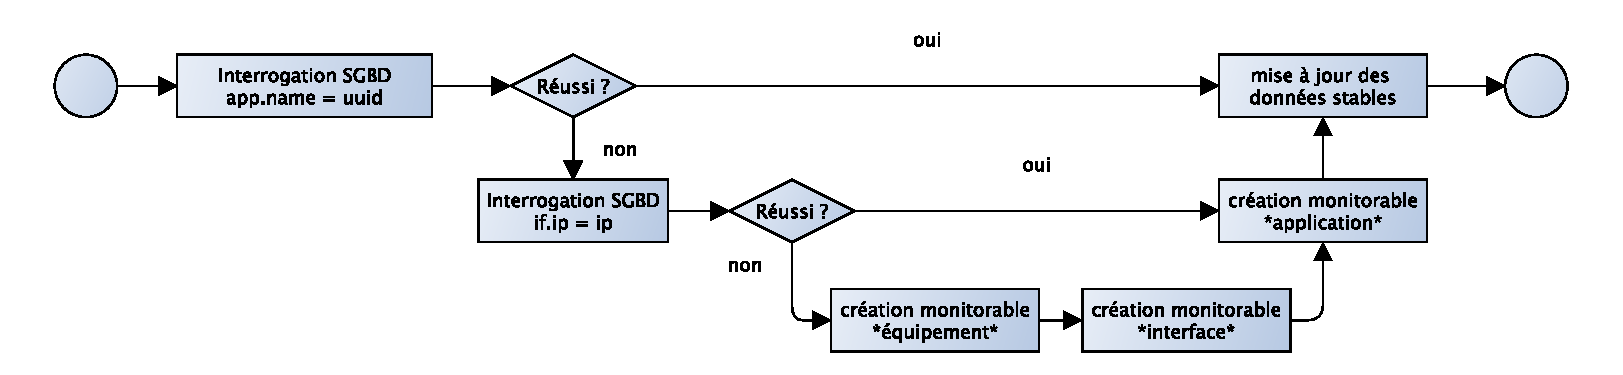
\includegraphics[width=\textwidth]{valid-domvision-statushandler}
	\caption{Description du processus de mise à jour de \textit{StatusSink}}\label{fig:valid:domvision:statushandler}
\end{figure}

Concernant les informations venant d'\textit{UPnP-DM}, nous pouvons regrouper tous les flux en un seul $DM$ grâce aux clés de jointures \textit{uuid} et \textit{SystemName}\footnote{Les sources sont synchronisés par le mécanisme d'événement. Sans cette synchronisation un partitionnement \textit{uuid} serait nécessaire.}. Ainsi, nous obtenons un flux indiquant que l'interface \textit{SystemName} (avec les propriétés données) est sur l'équipement identifié par le \textit{SerialNumber}. 
$$\begin{array}{c} DM(\textit{uuid},\textit{SerialNumber},\textit{SystemName},\textit{MACAddress},\textit{InterfaceType}, \textit{IPv4Address}, \t)\\
 DM = \IS(\textrm{Serial}[B] \Join \textrm{NetworkInterface}[B] \Join \textrm{IPInterface}[B])\end{array}$$
Nous pouvons appliquer la même approche que pour \textit{StatusHandler} en créant un composant puit \textit{DMSink} pour mettre à jour le catalogue grâce aux données de $DM$. La figure~\ref{fig:valid:domvision:cmshandler} résume le processus de ce puit.
\begin{figure}[ht]
        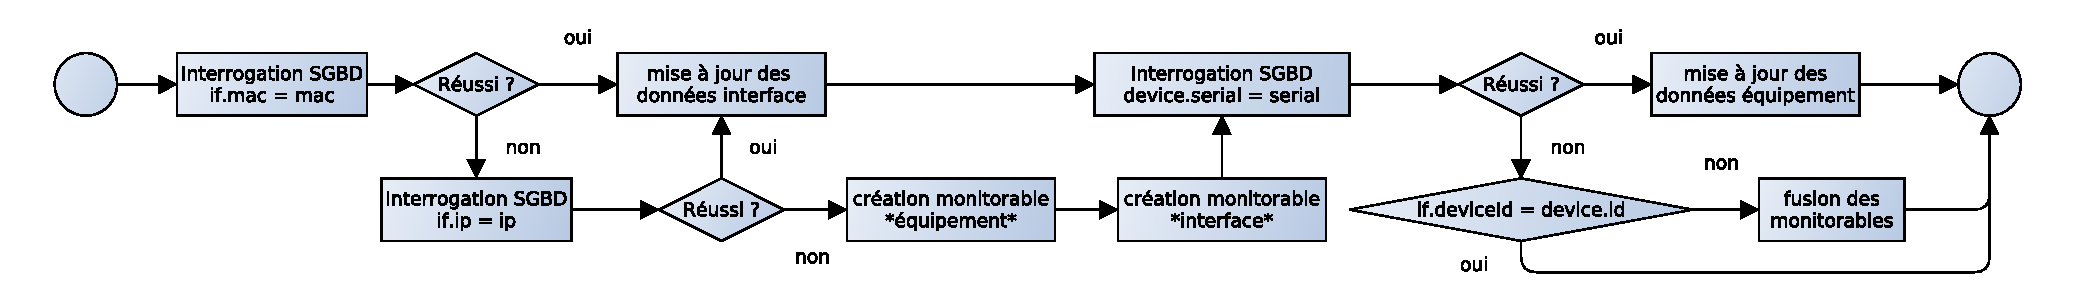
\includegraphics[width=\textwidth]{valid-domvision-cmshandler}
	\caption{Description du processus de mise à jour de \textit{DMSink}}\label{fig:valid:domvision:cmshandler}
\end{figure}

\subsection{Historisation des volatiles}\label{sec:valid:domvision:requetes:historisation}
Nous souhaitons maintenant archiver les données volatiles. Le premier point important à rappeler est que les flux donnés aux composants \textit{VolatilePersistence} doivent être identifiés, i.e. possèdent un attribut \textit{monitorableId}. Ainsi, le flux \textit{OperatingSystem} doit subir une opération pour transformer son \textit{uuid} en \textit{monitorableId} correspondant à l'\textit{équipement} qui le produit. La requête $CPUMem$ fournit le flux avec les attributs $A=$(\textit{CPUUsage}, \textit{MemoryUsage}, \textit{monitorableId},$\t$) répondant à ce problème :
$$CPUMem=\Pi_A \IS(\textit{OperatingSystem}[B]\ssjoin (\rho_{monitorableId/deviceId,uuid/name}\textit{Applications}\Join \textit{Monitorable}))$$

Ce flux est donné à une instance de \textit{VolatilePersistence} qui archive dans la table \textit{cpumemhistory} les données volatiles : \textit{cpu} et \textit{memory}. Nous pouvons noter que nous avons fait une jointure avec le catalogue sans difficultés.

Le flux \textit{IPUsage} ne nous donne pas les informations que nous souhaitons. En effet, nous voulons obtenir les données de débit, et le flux fournit un compteur d'octet. Toutefois, nous pouvons transformer une suite de comptage $(c_n,\t_n)$ en série de débits $(d_n,\t_n)$ par l'opération $d_n=\frac{c_n-c_{n-1}}{\t_n-\t_{n-1}}$. L'opérateur $\D_{t>t_0}^{(t,i)^-}$ est capable de revenir un \textit{batch} en arrière, ainsi la requête suivante\footnote{TotalBytesSent et TotalBytesReceived ont été renommés en tbs et tbr pour plus de facilité.} forme le flux voulu :
$$BandwidthUsage = \Pi_{...}\ \IS \left( e_{\frac{tbr-otbr}{\t-o\t}}^{bwr} e_{\frac{tbs-otbs}{\t-o\t}}^{bws}\left(IPUsage[B] \Join \D_{t>t_0}^{(t,i)^-} \rho_{\hspace{-0.33em}\mbox{\tiny $\begin{array}{l} otbs/tbs\\otbr/tbr\\ o\t/\t\end{array}$}}IPUsage[B]\right)\right)$$

Nous avons maintenant le flux possédant les données que nous souhaitons archiver. Comme pour \textit{CPUMem}, nous devons identifier l'entité sur laquelle nous enregistrons cette donnée. Ceci est faisable par une jointure semi-sensible sur la base de données en utilisant le \textit{uuid} de l'agent et le \textit{SystemName} représentant le \textit{nom} de l'interface. Cela produit un flux $Bandwidth$ que nous injectons dans un puit de persistance.

Les autres paramètres volatiles intéressants (changement d'\textit{IP} ou de \textit{status}...) s'enregistrent par le même procédé : extraire la ou les données à historiser ; identifier l'objet de rattachement.

Nous avons désormais un système d'observation capable d'entretenir sa vision du système et qui archive ses données volatiles. Ces données sont disponibles à travers le SGBD ce qui permet de faire diverses interrogations instantanées avec une capacité d'expression équivalente au \textit{SQL}. Ainsi, nous avons créé un panneau de contrôle indiquant la topologie du réseau ainsi que son histoire et des graphiques de métriques. Une série d'écran est disponible en annexe~\ref{misc:interface}.

\subsection{Formations d'alertes}\label{sec:valid:domvision:requetes:alerte}
Nous montrons maintenant quelques exemples de requêtes continues formant des alertes. La première est une simple sélection sur une valeur limite. Par exemple, nous pouvons supposer que les charges processeurs dépassant le seuil de 90\% sont à notifier à l'utilisateur. Nous pouvons raffiner ce critère par \enquote{\it la moyenne sur 1 minute supérieure à 90\%} afin de lisser les pics de valeurs. Nous pouvons exploiter le flux déjà prêt $CPUMem$ pour effectuer cette requête. Le nouveau flux est ensuite injecté à un composant puit de notification.
$$\IS\ \sigma_{avgcpu>90}(\null_{monitorableId}\G_{avg(CPUUsage)}^{avgcpu} CPUMem[T\ 1min\ 1min])$$

Afin de montrer les capacités d'interrogation de notre système, nous pouvons améliorer cette requête en exprimant le critère \enquote{\it la moyenne sur 1 minute est différente à 10\% près de la moyenne historique}. La valeur historique est obtenue par la relation temporelle produite par $HistAvgCPU=\null_{monitorableId}\G_{avg(cpu)}^{avgcpuhist} cpumemhistory$. Nous obtenons ainsi la requête :
$$\IS\ \sigma_{\abs{avgcpu-avghist}\geq 10}\left(AvgCPU\ssjoin HistAvgCPU\right)$$

Bien que cette requête mêle données historiques persistantes et données à la volée, nous sommes capables de l'écrire et de l'exécuter dans notre approche. Ceci prouve que notre approche est capable d'intégrer flux et relations persistantes par un langage semi-déclaratif.

\subsection{Journalisation du catalogue}
De plus, si l'utilisateur souhaite connaître les états passés du catalogue, il est possible de garder une trace dans le support persistant de tels changements. Prenons l'exemple de la relation \textit{Interfaces} du catalogue. Nous pouvons créer les flux d'insertion et de suppression de cette relation temporelle grâce à $\IS$ et $\DS$. Ainsi, un historique des changements de cette relation peut se traduire par :
$$InterfacesHist = \begin{cases} InterfacesIS = \IS(Interfaces) \\ InterfacesDS = \DS(Interfaces)\end{cases}$$
En persistant ces deux flux dans la base de donnée grâce à un puits de persistance, il est possible de reconstituer la relation \textit{Interfaces} à un temps quelconque $\tau$.

De plus, ces historiques permettent de fournir à l'utilisateur la liste des changements de son catalogue. Par exemple, il est possible de détailler une liste d'événements indiquant \enquote{\it un nouvel appareil vient de se connecter} ou \enquote{\it le profil de partage de contenu a disparu}. Ce type d'information sont très utiles dans le cadre du diagnostic afin de tracer au mieux les causes des problèmes.

Alternativement, il est possible d'archiver cette relation par l'utilisation de l'opérateur $\RSu$. Ceci permettra d'enregistrer l'ensemble de la relation à chaque changement. Nous remarquons que nous retrouvons le principe du calcul incrémental évoqué en section~\ref{sec:rw:sgfd:optimisation} en matérialisant une relation par l'ensemble de ses différences ou par l'ensemble de ses états.